\section{Tensor Network Simulation}\label{sec:tensor}
Tensors\cite{tensors} are mathematical objects with a lot in common with $n$-dimensional arrays. Some examples of tensors you are probably familiar with, a rank 0 tensor is just a scalar, a rank 1 tensor is a vector, a rank 2 tensor is a matrix, and so on. The rank of the tensor tells you how many indices you need to describe a single element in the tensor e.g., you need 1 index to tell which element in a vector you are talking about, and you need 2, namely a column and row index to uniquely specify an element in a matrix.  
Each index has a dimension, for example a rank 2 tensor that is $m$ by $n$ would have one index $i$ with dimension $n$ and another index $j$ with dimension $m$, we can then label an element in the tensor $a_{ij}$ where $i\in \{0,1,..,n-1\}, j\in \{0,1,..,m-1\}$. If we have more indices, they are sometimes written as $a_{ij}^{kl}$. 
We can use diagrams to draw these tensors, the tensors are represented by red squares and the indices are represented by lines attaching to the square. The shape and colour of the tensors and the position of the lines typically do not matter, what is important is which of them are connected by shared indices. 

\begin{figure}[H]
    \centering 
    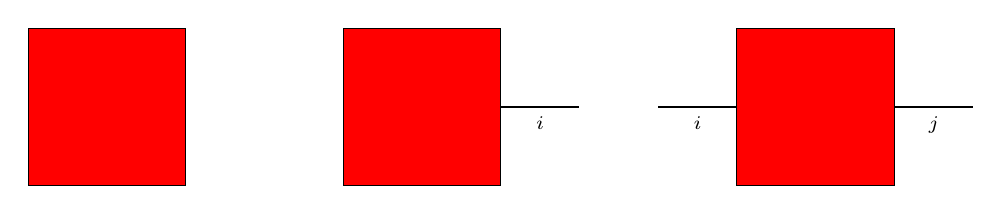
\begin{tikzpicture}
        \draw[fill=red] (-8,0) rectangle (-6,2) node[pos=0.5]{};

        \draw[fill=red] (-4,0) rectangle (-2,2) node[pos=0.5]{};
        \draw[](-2, 1) -- (-1, 1) 
         node[draw=none,fill=none,font=\scriptsize,midway,below]{$i$};
        \draw (-5, 1) node[draw=none]{};

        \draw[fill=red] (1,0) rectangle (3,2) node[pos=0.5]{};
        \draw[](3, 1) -- (4, 1)  
         node[draw=none,fill=none,font=\scriptsize,midway,below]{$j$};
        \draw[](1, 1) -- (0, 1)  
         node[draw=none,fill=none,font=\scriptsize,midway,below]{$i$};
        
    \end{tikzpicture}
    \caption{Rank 0, 1 and 2 tensors. Each index is represented by a line.}
    \label{fig:r2t}
\end{figure}

\noindent
Often the indices are not labelled on these drawings. If we have two tensors, we can make them share an index if they each have an index with the same dimension. So, if we have two rank 3 tensors, one where the dimensions of the indexes are $2, 3, 5$ and another where the dimensions are $1, 4, 3$, we can see that they both have an index of dimension 3 so if we wish we can make them share label for this index. Thus, they could have the indices $i, j, k$ and $l, m, j$, notice the reuse of $j$. 

\begin{figure}[H]
    \centering 
    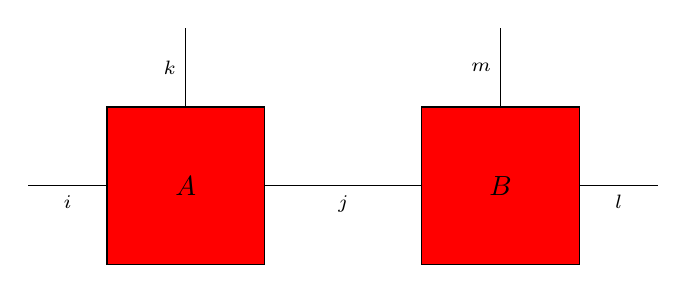
\begin{tikzpicture}
        \draw[fill=red] (0,0) rectangle (2,2) node[pos=0.5]{$A$};
        \draw[](2, 1) -- (3, 1)  
         node[draw=none,fill=none,font=\scriptsize,midway,below]{};
        \draw[](0, 1) -- (-1, 1)  
         node[draw=none,fill=none,font=\scriptsize,midway,below]{$i$};
        \draw[](1, 2) -- (1, 3)  
         node[draw=none,fill=none,font=\scriptsize,midway,left]{$k$};
        
        \draw[fill=red](4,0) rectangle (6,2) node[pos=0.5]{$B$};
        \draw[](6, 1) -- (7, 1)  
         node[draw=none,fill=none,font=\scriptsize,midway,below]{$l$};
        \draw[](4, 1) -- (3, 1)  
         node[draw=none,fill=none,font=\scriptsize,below]{$j$};
        \draw[](5, 2) -- (5, 3)  
         node[draw=none,fill=none,font=\scriptsize,midway,left]{$m$};
    \end{tikzpicture}
    \caption{Rank 3 tensors sharing index $j$.}
    \label{fig:2r3t}
\end{figure}
\subsection{Contracting tensors }
\noindent
But what is this good for? In essence, when we make tensors share indices it is a way to symbolise that we are \textit{contracting} them. The actual computation of the contraction can be done at a later point we are just marking our intention. This is important as we might want to build an entire network of tensors and then be strategic about which shared indices we choose to contract. Contracting a shared index is synonymous with computing the product of the two tensors. 
\begin{figure}[H]
    \centering 
    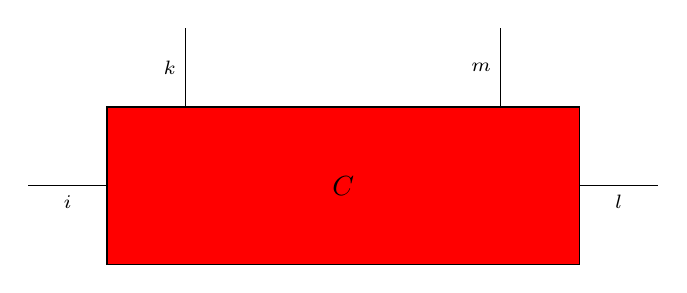
\begin{tikzpicture}
        \draw[fill=red](0,0) rectangle (6,2) node[pos=0.5]{$C$};
        \draw[](0, 1) -- (-1, 1)  
         node[draw=none,fill=none,font=\scriptsize,midway,below]{$i$};
        \draw[](1, 2) -- (1, 3)  
         node[draw=none,fill=none,font=\scriptsize,midway,left]{$k$};
        
        \draw[](6, 1) -- (7, 1)  
         node[draw=none,fill=none,font=\scriptsize,midway,below]{$l$};
        \draw[](5, 2) -- (5, 3)  
         node[draw=none,fill=none,font=\scriptsize,midway,left]{$m$};
    \end{tikzpicture}
    \caption{Rank 4 tensor after contracting shared index $j$ from Figure \ref{fig:2r3t}.}
    \label{fig:4t}
\end{figure}
\noindent
In this example we have two tensors A and B where each have elements of the form $a_{ijk}, b_{lmj}$ resulting in a single tensor C with the elements $$c_{iklm}=\displaystyle\sum_{x=0}^{dim(j)-1} a_{ixk}b_{lmx} $$
Here $dim(j)=3$ and we subtract 1 since the elements are 0 indexed. In \textit{tensor notation} the summation is implicit if there is a shared index in such an equation so we would just write $c_{iklm}=a_{ijk}b_{lmj}$

\subsection{Reshaping tensors }
\noindent 
$\ket{\Psi}$ is a vector, in other words a rank 1 tensor, but later we are using them as rank 2 and 3 tensors, how can we do so? We can simply add some ranks like so,
$\ket{\Psi} \rightarrow
\begin{bmatrix}
    \ket{\Psi}
\end{bmatrix} \rightarrow
\begin{bmatrix}
    \begin{bmatrix}
        \ket{\Psi}
    \end{bmatrix}
\end{bmatrix}$, this can be done for the gates as well; we just add indices with dimension 1.  
The more general rule goes that you can change the rank of the tensor as much as you want as long as the product of the dimensions is the same. By this logic we can always add indices with dimension 1, but we can also split indices in two as long as the product of the dimensions of the new indices equals the old index's dimensions. We can also combine indices. This operation is often called reshaping.  

\subsection{Splitting two qubit gates into two tensors with a shared index }
The SVD\cite{SVD} is a mathematical operation that disassembles a matrix A into a matrix U, a vector of singular values $\lambda$ and a matrix V, which upholds the property $A=U\Lambda Vh$ where $\Lambda$ is a matrix where the diagonal corresponds to the values of $\lambda$ and all the other elements are 0, and Vh is the conjugate transpose of V. 


\vspace{\baselineskip}
\noindent
To take advantage of this we have our 4x4 gates, they have two indices that each have a dimension 4 but we reshape to 4 indices with dimensions 2 - an input for each qubit and an output for each. So if we describe our matrix elements with regards to these indices we can say an element $a_{i_1i_2o_1o_2}$ is in either the top half or the bottom half depending on $i_1$, and in the left half or right half depending on $o_1$ this gives us a sub matrix that is 2x2, which we divide the same way using $i_2$ and $o_2$. So, our matrix elements are divided like this: 
\begin{figure}[H]
    $$
    \begin{bmatrix}
        a_{0000} & a_{0001} & a_{0010} & a_{0011}\\
        a_{0100} & a_{0101} & a_{0110} & a_{0111}\\
        a_{1000} & a_{1001} & a_{1010} & a_{1011}\\
        a_{1100} & a_{1101} & a_{1110} & a_{1111}\\
    \end{bmatrix}
    $$
    \caption{Matrix element indices.}
    \label{fig:matrix_indices}
\end{figure}
\noindent
Unfortunately, the SVD splits vertically i.e., in this case we would be splitting the gate between the inputs and outputs, but we are interested in splitting between the two qubits, so $i_1$ and $o_1$ are separate from $i_2$ and $o_2$. Luckily, we can just swap around the indices and thus elements beforehand, we just have to remember to swap them back when all is set and done.
\begin{figure}[H]
    $$
    \begin{bmatrix}
        a_{0000} & a_{0001} & a_{0100} & a_{0101}\\
        a_{0010} & a_{0011} & a_{0110} & a_{0111}\\
        a_{1000} & a_{1001} & a_{1100} & a_{1101}\\
        a_{1010} & a_{1011} & a_{1110} & a_{1111}\\
    \end{bmatrix}
    $$
    \caption{Indices swapped.}
    \label{fig:matrix_swapped}
\end{figure}

\begin{figure}[H]
    \centering 
    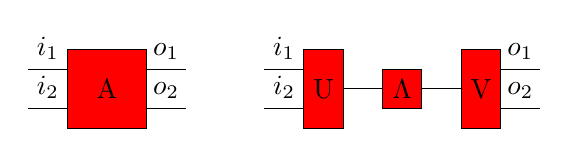
\begin{tikzpicture}
        \draw[] (-3,0.25) -- (-2.5,0.25) node[midway,above]{$i_2$};
        \draw[] (-3,0.75) -- (0.5-3,0.75) node[midway,above]{$i_1$};
        \draw[fill=red] (0.5-3,0) rectangle (-1.5,1) node[pos=0.5]{A};
        \draw[] (2-3.5,0.25) -- (2.5-3.5,0.25) node[midway,above]{$o_2$};
        \draw[] (2-3.5,0.75) -- (2.5-3.5,0.75) node[midway,above]{$o_1$};

        \draw[] (0,0.25) -- (0.5,0.25) node[midway,above]{$i_2$};
        \draw[] (0,0.75) -- (0.5,0.75) node[midway,above]{$i_1$};
        \draw[fill=red] (0.5,0) rectangle (1,1) node[pos=0.5]{U};
        \draw[] (1,0.5) -- (1.5,0.5);
        \draw[fill=red] (1.5,0.25) rectangle (2,0.75) node[pos=0.5]{$\Lambda$};
        \draw[] (2,0.5) -- (2.5,0.5);
        \draw[fill=red] (2.5,0) rectangle (3,1) node[pos=0.5]{V};
        \draw[] (3,0.25) -- (3.5,0.25) node[midway,above]{$o_2$};
        \draw[] (3,0.75) -- (3.5,0.75) node[midway,above]{$o_1$};
    \end{tikzpicture}
    \caption{SVD without swapping.}
    \label{fig:svd_no_swap}
\end{figure}
\begin{figure}[H]
    \centering 
    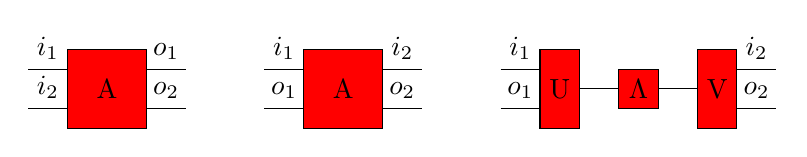
\begin{tikzpicture}
        \draw[] (-3-3,0.25) -- (-2.5-3,0.25) node[midway,above]{$i_2$};
        \draw[] (-3-3,0.75) -- (0.5-3-3,0.75) node[midway,above]{$i_1$};
        \draw[fill=red] (0.5-3-3,0) rectangle (-1.5-3,1) node[pos=0.5]{A};
        \draw[] (2-3.5-3,0.25) -- (2.5-3.5-3,0.25) node[midway,above]{$o_2$};
        \draw[] (2-3.5-3,0.75) -- (2.5-3.5-3,0.75) node[midway,above]{$o_1$};

        \draw[] (-3,0.25) -- (-2.5,0.25) node[midway,above]{$o_1$};
        \draw[] (-3,0.75) -- (0.5-3,0.75) node[midway,above]{$i_1$};
        \draw[fill=red] (0.5-3,0) rectangle (-1.5,1) node[pos=0.5]{A};
        \draw[] (2-3.5,0.25) -- (2.5-3.5,0.25) node[midway,above]{$o_2$};
        \draw[] (2-3.5,0.75) -- (2.5-3.5,0.75) node[midway,above]{$i_2$};

        \draw[] (0,0.25) -- (0.5,0.25) node[midway,above]{$o_1$};
        \draw[] (0,0.75) -- (0.5,0.75) node[midway,above]{$i_1$};
        \draw[fill=red] (0.5,0) rectangle (1,1) node[pos=0.5]{U};
        \draw[] (1,0.5) -- (1.5,0.5);
        \draw[fill=red] (1.5,0.25) rectangle (2,0.75) node[pos=0.5]{$\Lambda$};
        \draw[] (2,0.5) -- (2.5,0.5);
        \draw[fill=red] (2.5,0) rectangle (3,1) node[pos=0.5]{V};
        \draw[] (3,0.25) -- (3.5,0.25) node[midway,above]{$o_2$};
        \draw[] (3,0.75) -- (3.5,0.75) node[midway,above]{$i_2$};
    \end{tikzpicture}
    \caption{SVD with swapping.}
    \label{fig:svd_swap}
\end{figure}
\noindent
We do though want to express this using two tensors only, but this is fortunately easy as we can just split $\Lambda$ by squaring every value in it. Now we can contract two indices and get the result we want. 
\begin{figure}[H]
    \centering 
    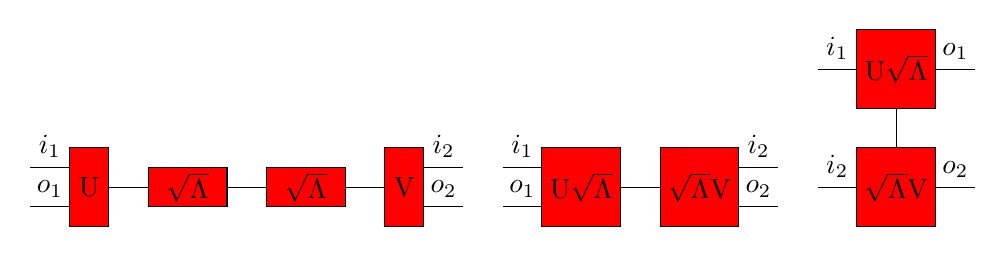
\begin{tikzpicture}
        \draw[] (0,0.25) -- (0.5,0.25) node[midway,above]{$o_1$};
        \draw[] (0,0.75) -- (0.5,0.75) node[midway,above]{$i_1$};
        \draw[fill=red] (0.5,0) rectangle (1,1) node[pos=0.5]{U};
        \draw[] (1,0.5) -- (1.5,0.5);
        \draw[fill=red] (1.5,0.25) rectangle (2+0.5,0.75) node[pos=0.5]{$\sqrt{\Lambda}$};
        \draw[] (2.5,0.5) -- (2.5+0.5,0.5);
        \draw[fill=red] (1.5+1.5,0.25) rectangle (2+2,0.75) node[pos=0.5]{$\sqrt{\Lambda}$};
        \draw[] (2+2,0.5) -- (2.5+2,0.5);
        \draw[fill=red] (2.5+2,0) rectangle (3+2,1) node[pos=0.5]{V};
        \draw[] (3+2,0.25) -- (3.5+2,0.25) node[midway,above]{$o_2$};
        \draw[] (3+2,0.75) -- (3.5+2,0.75) node[midway,above]{$i_2$};

        \draw[] (4+2,0.25) -- (4.5+2,0.25) node[midway,above]{$o_1$};
        \draw[] (4+2,0.75) -- (4.5+2,0.75) node[midway,above]{$i_1$};
        \draw[fill=red] (4.5+2,0) rectangle (5.5+2,1) node[pos=0.5]{U$\sqrt{\Lambda}$};
        \draw[] (1+4+2+0.5,0.5) -- (1.5+4+2+0.5,0.5);
        \draw[fill=red] (5.5+0.5+2,0) rectangle (6.5+0.5+2,1) node[pos=0.5]{$\sqrt{\Lambda}$V};
        \draw[] (6.5+0.5+2,0.25) -- (7+2+0.5,0.25) node[midway,above]{$o_2$};
        \draw[] (6.5+2+0.5,0.75) -- (9.5,0.75) node[midway,above]{$i_2$};

        \draw[] (10,0.5) -- (10.5,0.5) node[midway,above]{$i_2$};
        \draw[] (10,2) -- (10.5,2) node[midway,above]{$i_1$};
        \draw[fill=red] (10.5,0) rectangle (11.5,1) node[pos=0.5]{$\sqrt{\Lambda}$V};
        \draw[] (11,1) -- (11,1.5);
        \draw[fill=red] (10.5,1.5) rectangle (11.5,2.5) node[pos=0.5]{U$\sqrt{\Lambda}$};
        \draw[] (11.5,0.5) -- (12,0.5) node[midway,above]{$o_2$};
        \draw[] (11.5,2) -- (12,2) node[midway,above]{$o_1$};

    \end{tikzpicture}
    \caption{Combine the network from figure \ref{fig:svd_swap} into two tensors.}
    \label{fig:svd_combine}
\end{figure}
\noindent
This whole process is sometimes called the operator Schmidt decomposition\cite{osd}.  

\subsection{representing a circuit and state using tensors}
\noindent
We can use a tensor network to represent our $QFT$ circuit and our state. We will use a matrix product state (MPS) to represent our state, and a matrix product operator (MPO) to represent our circuit, these are just subcategories of tensor networks. 

\begin{figure}[H]
    \centering 
    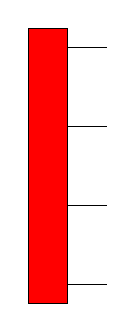
\begin{tikzpicture}
        \draw[] (0.25,-1) -- (0.25,-4);
        \foreach \i in {1,...,4}
        {
                \draw[](0.5, -\i +0.25) -- (1, -\i +0.25); 
        }
        \draw[fill=red] (0,-0.5) rectangle (0.5,-4) node[pos=0.5]{};
    \end{tikzpicture}
    \caption{4-qubit state represented as a tensor (MPS).}
    \label{fig:psi4t}
\end{figure}
\noindent
Here we have the whole state in one large tensor. This is highly undesirable as this uses a lot of memory, we would rather construct a network of tensors. Let us take the state $\ket{0010}$ as an example.
\begin{figure}[H]
    \centering 
    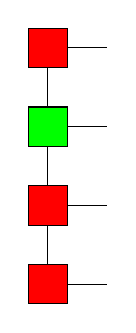
\begin{tikzpicture}
        \draw[] (0.25,-1) -- (0.25,-4);
        \foreach \i in {1,...,4}
        {
                \draw[](0.5, -\i +0.25) -- (1, -\i +0.25); 
                \draw[fill=red] (0,-\i) rectangle (0.5,-\i+0.5) node[pos=0.5]{};
        }
        \draw[fill=green] (0,-2) rectangle (0.5,-2+0.5) node[pos=0.5]{};
    \end{tikzpicture}
    \caption{4-qubit state $\ket{0010}$ represented as a tensor network (MPS). Red represents $\ket{0}$ and green $\ket{1}$. }
    \label{fig:psi4t_mps}
\end{figure}
\noindent
Here we reshape the tensors representing each qubit to fit with our network structure. They simply have shared indices of size 1 connecting them. 
Now let us look at representing the QFT as a MPO:
\begin{figure}[H]
    \centering 
    \scalebox{0.57}{
    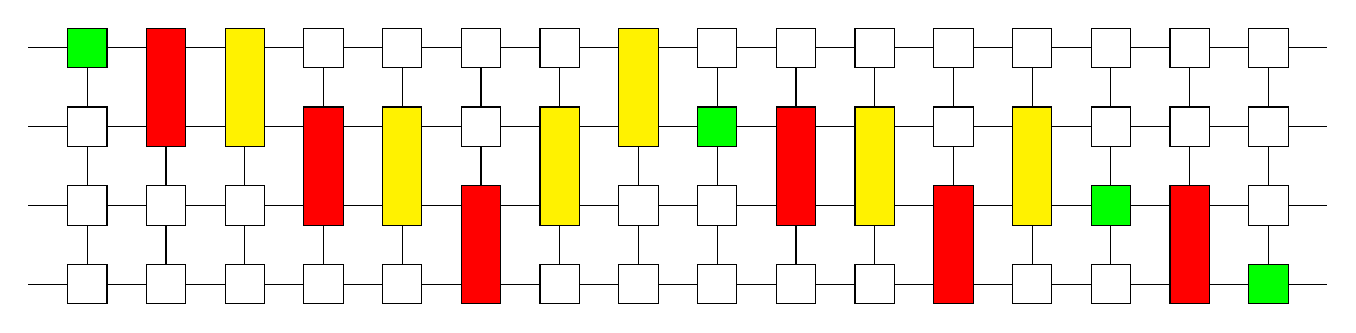
\begin{tikzpicture}
        \foreach \j in {0,...,15}{
            \draw[](\j+0.25,0) -- (\j+0.25, -3);
        }
        \foreach \i in {0,...,3}
        {
            \draw[](-0.5,-0.25-\i) -- (16, -0.25-\i);
            \foreach \j in {0,...,15}{
                \draw[fill=white] (\j,-\i) rectangle (0.5+\j,-0.5-\i) node[pos=0.5]{};
            }
        }

        \draw[fill=green] (0,0) rectangle (0.5,-0.5) node[pos=0.5]{};
        \foreach \i in {0,...,1}
        {
            \draw[fill=red] (1+\i+\i,-\i) rectangle (0.5+1+\i+\i,-0.5-1-\i) node[pos=0.5]{};
            \draw[fill=yellow] (2+\i+\i,-\i) rectangle (0.5+2+\i+\i,-0.5-1-\i) node[pos=0.5]{};
        }
        \draw[fill=red] (5,-2) rectangle (0.5+1+4,-0.5-1-2) node[pos=0.5]{};
        \draw[fill=yellow] (6,-1) rectangle (0.5+2+4,-0.5-1-1) node[pos=0.5]{};
        \draw[fill=yellow] (7,0) rectangle (0.5+2+5,-0.5-1) node[pos=0.5]{};

        \draw[fill=green] (8,-1) rectangle (0.5+8,-0.5-1) node[pos=0.5]{};
        \draw[fill=red] (9,-1) rectangle (0.5+9,-0.5-1-1) node[pos=0.5]{};
        \draw[fill=yellow] (10,-1) rectangle (0.5+10,-0.5-1-1) node[pos=0.5]{};
        \draw[fill=red] (11,-2) rectangle (0.5+11,-0.5-1-2) node[pos=0.5]{};
        \draw[fill=yellow] (12,-1) rectangle (0.5+12,-0.5-1-1) node[pos=0.5]{};

        \draw[fill=green] (13,-2) rectangle (0.5+13,-0.5-2) node[pos=0.5]{};
        \draw[fill=red] (14,-2) rectangle (0.5+14,-0.5-1-2) node[pos=0.5]{};

        \draw[fill=green] (15,-3) rectangle (0.5+15,-0.5-3) node[pos=0.5]{};
    \end{tikzpicture}
    }
    \caption{$QFT_4$ represented as a tensor network (MPO). White represents an identity gate, green a Hadamard gate, red a controlled $R_x,x\in \{2,3,4\}$ gate, and yellow a swap gate.}
    \label{fig:qft4t}
\end{figure}
\noindent
Now you might ask why we suddenly are using a ton of swap gates, and what are they even. Swap gates simply swap the values of two qubits, so if $\ket{10}$ goes in $\ket{01}$ comes out. This is simulated with this matrix, when swapping adjacent qubits as we are. 
\begin{figure}[H]
    \centering
    $$
    \begin{bmatrix}
        1 & 0 & 0 & 0\\ 
        0 & 0 & 1 & 0\\ 
        0 & 1 & 0 & 0\\ 
        0 & 0 & 0 & 1\\ 
    \end{bmatrix}
    $$
    \caption{SWAP gate matrix. }
    \label{fig:swap}
\end{figure}

\noindent
We do this to avoid having non-local gates in the circuit, such as the controlled $R_x$ gates we use in the QFT. This was not a concern when doing the dense simulation, but here we have to split everything up into tensors acting on individual qubits and therefore would like smaller gates to start with. The reason we have to split everything up is mostly a limitation of the library\cite{quimb} we are using for the simulation; it is a perfectly valid tensor network even without splitting every gate. It does add a cost of slightly less than two swap gates per non-local gate.  
This low overhead is not something that can be achieved in general, the most general way to make every gate local requires swapping the two qubits with the ones between them until they are adjacent, applying the gate, and then swapping them back to where they came from, this takes swap gates equal to the number of qubits between the two target qubits times two. We are fortunately in a situation where we can do this in a smarter way. 
\begin{figure}[H]
    \centering 
    \scalebox{0.57}{
    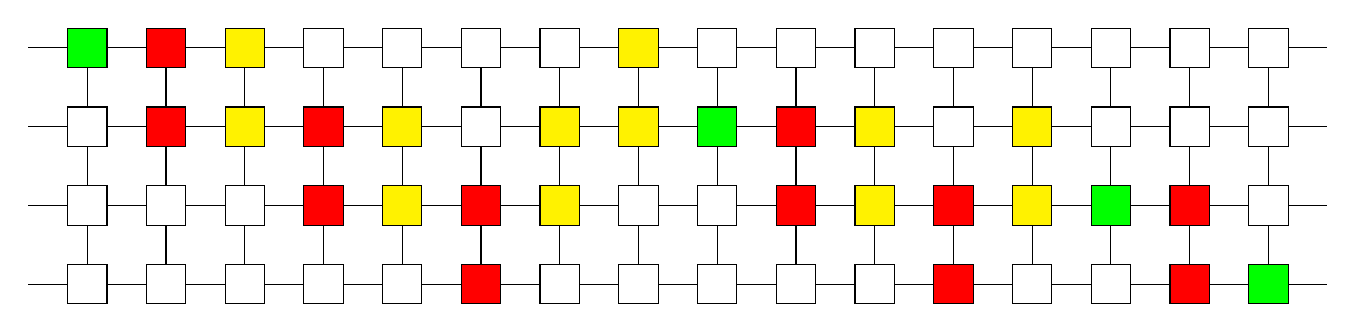
\begin{tikzpicture}
        \foreach \j in {0,...,15}{
            \draw[](\j+0.25,0) -- (\j+0.25, -3);
        }
        \foreach \i in {0,...,3}
        {
            \draw[](-0.5,-0.25-\i) -- (16, -0.25-\i);
            \foreach \j in {0,...,15}{
                \draw[fill=white] (\j,-\i) rectangle (0.5+\j,-0.5-\i) node[pos=0.5]{};
            }
        }

        \draw[fill=green] (0,0) rectangle (0.5,-0.5) node[pos=0.5]{};
        \foreach \i in {0,...,1}
        {
            \draw[fill=red] (1+\i+\i,-\i) rectangle (0.5+1+\i+\i,-0.5-\i) node[pos=0.5]{};
            \draw[fill=red] (1+\i+\i,-\i-1) rectangle (0.5+1+\i+\i,-0.5-1-\i) node[pos=0.5]{};
            \draw[fill=yellow] (2+\i+\i,-\i) rectangle (0.5+2+\i+\i,-0.5-\i) node[pos=0.5]{};
            \draw[fill=yellow] (2+\i+\i,-\i-1) rectangle (0.5+2+\i+\i,-0.5-1-\i) node[pos=0.5]{};
        }
        \draw[fill=red] (5,-2) rectangle (0.5+1+4,-0.5-2) node[pos=0.5]{};
        \draw[fill=red] (5,-3) rectangle (0.5+1+4,-0.5-1-2) node[pos=0.5]{};
        \draw[fill=yellow] (6,-1) rectangle (0.5+2+4,-0.5-1) node[pos=0.5]{};
        \draw[fill=yellow] (6,-2) rectangle (0.5+2+4,-0.5-1-1) node[pos=0.5]{};
        \draw[fill=yellow] (7,0) rectangle (0.5+2+5,-0.5) node[pos=0.5]{};
        \draw[fill=yellow] (7,-1) rectangle (0.5+2+5,-0.5-1) node[pos=0.5]{};

        \draw[fill=green] (8,-1) rectangle (0.5+8,-0.5-1) node[pos=0.5]{};
        \draw[fill=red] (9,-1) rectangle (0.5+9,-0.5-1) node[pos=0.5]{};
        \draw[fill=red] (9,-2) rectangle (0.5+9,-0.5-1-1) node[pos=0.5]{};
        \draw[fill=yellow] (10,-1) rectangle (0.5+10,-0.5-1) node[pos=0.5]{};
        \draw[fill=yellow] (10,-2) rectangle (0.5+10,-0.5-1-1) node[pos=0.5]{};
        \draw[fill=red] (11,-2) rectangle (0.5+11,-0.5-2) node[pos=0.5]{};
        \draw[fill=red] (11,-3) rectangle (0.5+11,-0.5-1-2) node[pos=0.5]{};
        \draw[fill=yellow] (12,-1) rectangle (0.5+12,-0.5-1) node[pos=0.5]{};
        \draw[fill=yellow] (12,-2) rectangle (0.5+12,-0.5-1-1) node[pos=0.5]{};

        \draw[fill=green] (13,-2) rectangle (0.5+13,-0.5-2) node[pos=0.5]{};
        \draw[fill=red] (14,-2) rectangle (0.5+14,-0.5-2) node[pos=0.5]{};
        \draw[fill=red] (14,-3) rectangle (0.5+14,-0.5-1-2) node[pos=0.5]{};

        \draw[fill=green] (15,-3) rectangle (0.5+15,-0.5-3) node[pos=0.5]{};
    \end{tikzpicture}
    }
    \caption{$QFT_4$ from figure \ref{fig:qft4t} with all two qubit gates split using the operator Schmidt decomposition.}
    \label{fig:qft4t_svd}
\end{figure} 
\begin{figure}[H]
    \centering 
    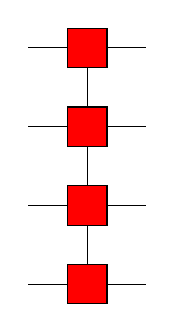
\begin{tikzpicture}
        \draw[] (0.25,-1) -- (0.25,-4);
        \foreach \i in {1,...,4}
        {
            \draw[](-0.5, -\i +0.25) -- (1, -\i +0.25); 
            \draw[fill=red] (0,-\i) rectangle (0.5,-\i+0.5) node[pos=0.5]{};
        }
    \end{tikzpicture}
    \caption{$QFT_4$ from figure \ref{fig:qft4t_svd} with 'horizontal' shared indices contracted.}
    \label{fig:mpo}
\end{figure}
\noindent 
We have used the operator Schmidt decomposition to split the two qubit gates such that we can apply them to each of our qubits separately.  
\noindent
Now that we have our state MPS and our QFT MPO we can apply the MPO to the MPS by connecting the outputs from the MPS to the inputs of the MPO and contracting those shared indexes. This results in an updated MPS. If we wish to combine two MPOs into one we do the same, just connecting the output of one to the input of another and contracting. 

\begin{figure}[H]
    \centering 
    \begin{subfigure}{.3\textwidth}
        \centering
        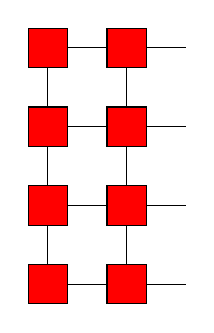
\begin{tikzpicture}
            \draw[] (0.25,-1) -- (0.25,-4);
            \draw[] (-0.75,-1) -- (-0.75,-4);
            \foreach \i in {1,...,4}
            {
                    \draw[](-0.5, -\i +0.25) -- (1, -\i +0.25); 
                    \draw[fill=red] (0,-\i) rectangle (0.5,-\i+0.5) node[pos=0.5]{};
                    \draw[fill=red] (-1,-\i) rectangle (-0.5,-\i+0.5) node[pos=0.5]{};
            }
        \end{tikzpicture}
        \caption{Before contraction.}
    \end{subfigure}%
    \begin{subfigure}{.2\textwidth}
      \centering
        $\iff$
        \vspace{5em}
    \end{subfigure}
    \begin{subfigure}{.3\textwidth}
        \hspace{2em}
        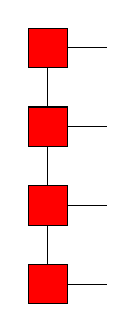
\begin{tikzpicture}
            \draw[] (0.25,-1) -- (0.25,-4);
            \foreach \i in {1,...,4}
            {
                    \draw[](0.5, -\i +0.25) -- (1, -\i +0.25); 
                    \draw[fill=red] (0,-\i) rectangle (0.5,-\i+0.5) node[pos=0.5]{};
            }
        \end{tikzpicture}
        \caption{After contraction.}
    \end{subfigure}%
    \caption{MPO applied to MPS.}
    \label{fig:mpo_mps}
\end{figure}

\noindent
After splitting a gate which acts on more than one qubit the index, they share will have a dimension of 1 or larger, and when we contract a MPO like so, we can see that the dimension scales quite quickly, with the layers if we do not do something: 
\begin{figure}[H]
    \centering 
    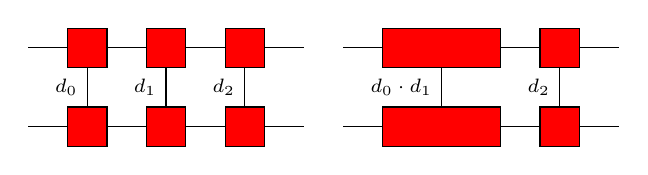
\begin{tikzpicture}
        \foreach \j in {0,...,2}
        {
            \foreach \i in {1,...,2}
            {
                \draw[](-0.5+\j, -\i +0.25) -- (1+\j, -\i +0.25) node[font=\scriptsize,below,pos=0.9]{};
 
                \draw[fill=red] (0+\j,-\i) rectangle (0.5+\j,-\i+0.5) node[pos=0.5]{};
            }
            \foreach \i in {1,...,1}
            {
                \draw[] (0.25+\j,-\i) -- (0.25+\j,-\i-0.5) node[font=\scriptsize,midway,left]{$d_{\j}$};
            }
        }
        \foreach \j in {4,...,5}
        {
        }
        \foreach \i in {1,...,2}
        {
            \draw[](-0.5+6, -\i +0.25) -- (1+6, -\i +0.25); 
            \draw[fill=red] (0+6,-\i) rectangle (0.5+6,-\i+0.5) node[pos=0.5]{};
        }
        \foreach \i in {1,...,2}
        {
            \draw[](-0.5+4, -\i +0.25) -- (1+5, -\i +0.25); 
            \draw[fill=red] (0+4,-\i) rectangle (0.5+5,-\i+0.5) node[pos=0.5]{};
        }
        \draw[] (0.25+4.5,-1) -- (0.25+4.5,-1-0.5) node[font=\scriptsize,midway,left]{$d_{0}\cdot d_{1}$};
        \draw[] (0.25+6,-1) -- (0.25+6,-1-0.5) node[font=\scriptsize,midway,left]{$d_{2}$};
    \end{tikzpicture}

    \caption{MPO with vertical bond dimensions $d_{i}.$}
    \label{fig:mpo_contraction}
\end{figure}
\noindent 
So, what can we do? We can compress the bonds in our MPO every now and then, to get them back to a manageable size, this is possible since we know our QFT has a fixed max bond dimension. The way we do it is to go through our bonds, e.g. from top to bottom and contract then re-split them using the SVD. This will help, but we can do better if we are willing to pay a little accuracy, we can truncate the singular values to only the ones that contribute the most and cut out those that do not contribute a lot to the result. In the QFT circuit it has been shown that the singular values decrease exponentially so we don't lose much precission.    

\begin{figure}[H]
    \centering
    \scalebox{0.3}{
    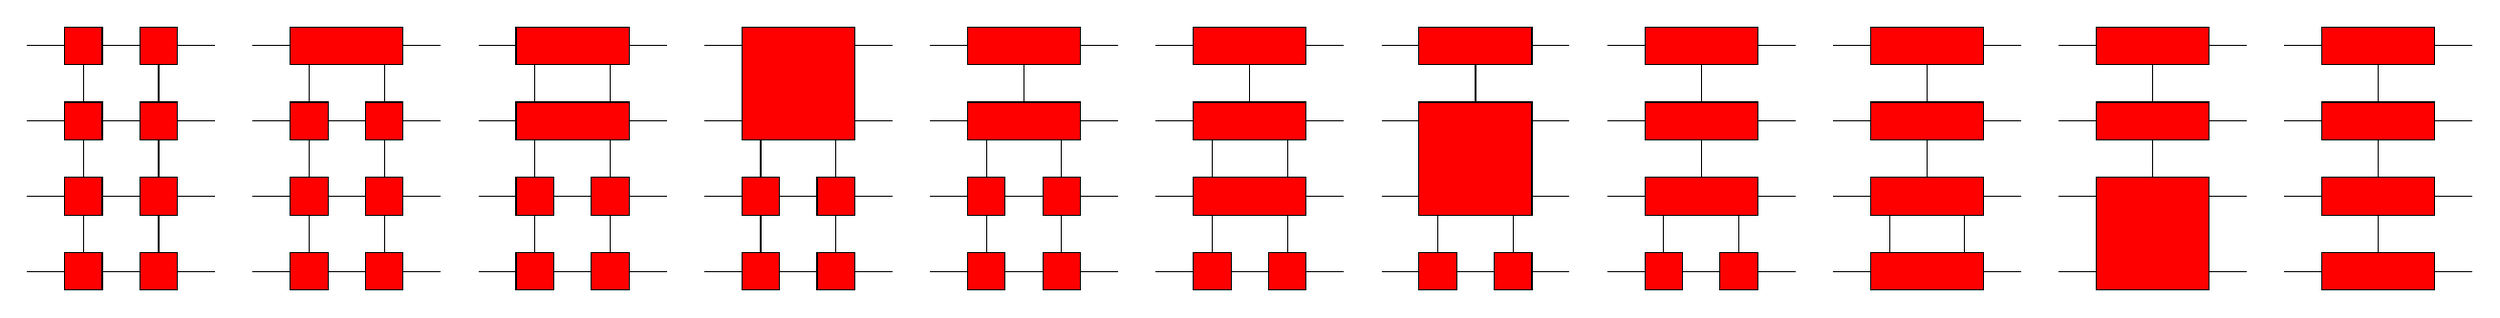
\begin{tikzpicture}
        \foreach \j in {0,...,1}
        {
            \draw[] (0.25+\j,-1) -- (0.25+\j,-4);
            \foreach \i in {1,...,4}
            {
                \draw[](-0.5+\j, -\i +0.25) -- (1+\j, -\i +0.25); 
                \draw[fill=red] (0+\j,-\i) rectangle (0.5+\j,-\i+0.5) node[pos=0.5]{};
            }
        }
        \foreach \j in {3,...,4}
        {
            \draw[] (0.25+\j,-1) -- (0.25+\j,-4);
            \foreach \i in {1,...,4}
            {
                \draw[](-0.5+\j, -\i +0.25) -- (1+\j, -\i +0.25); 
                \draw[fill=red] (0+\j,-\i) rectangle (0.5+\j,-\i+0.5) node[pos=0.5]{};
            }
        }
        \draw[fill=red] (0+3,-1) rectangle (0.5+4,-1+0.5) node[pos=0.5]{};
        \foreach \j in {6,...,7}
        {
            \draw[] (0.25+\j,-1) -- (0.25+\j,-4);
            \foreach \i in {1,...,4}
            {
                \draw[](-0.5+\j, -\i +0.25) -- (1+\j, -\i +0.25); 
                \draw[fill=red] (0+\j,-\i) rectangle (0.5+\j,-\i+0.5) node[pos=0.5]{};
            }
        }
        \draw[fill=red] (0+6,-1) rectangle (0.5+7,-1+0.5) node[pos=0.5]{};
        \draw[fill=red] (0+6,-2) rectangle (0.5+7,-2+0.5) node[pos=0.5]{};
        \foreach \j in {9,...,10}
        {
            \draw[] (0.25+\j,-1) -- (0.25+\j,-4);
            \foreach \i in {1,...,4}
            {
                \draw[](-0.5+\j, -\i +0.25) -- (1+\j, -\i +0.25); 
                \draw[fill=red] (0+\j,-\i) rectangle (0.5+\j,-\i+0.5) node[pos=0.5]{};
            }
        }
        \draw[fill=red] (0+9,-0.5) rectangle (0.5+10,-2) node[pos=0.5]{};
        \foreach \j in {12,...,13}
        {
            \draw[] (0.25+\j,-2) -- (0.25+\j,-4);
            \foreach \i in {1,...,4}
            {
                \draw[](-0.5+\j, -\i +0.25) -- (1+\j, -\i +0.25); 
                \draw[fill=red] (0+\j,-\i) rectangle (0.5+\j,-\i+0.5) node[pos=0.5]{};
            }
        }
        \draw[] (0.75+12,-1) -- (0.75+12,-2);
        \draw[fill=red] (0+12,-1) rectangle (0.5+13,-1+0.5) node[pos=0.5]{};
        \draw[fill=red] (0+12,-2) rectangle (0.5+13,-2+0.5) node[pos=0.5]{};
        \foreach \j in {15,...,16}
        {
            \draw[] (0.25+\j,-2) -- (0.25+\j,-4);
            \foreach \i in {1,...,4}
            {
                \draw[](-0.5+\j, -\i +0.25) -- (1+\j, -\i +0.25); 
                \draw[fill=red] (0+\j,-\i) rectangle (0.5+\j,-\i+0.5) node[pos=0.5]{};
            }
        }
        \draw[] (0.75+15,-1) -- (0.75+15,-2);
        \draw[fill=red] (0+15,-1) rectangle (0.5+16,-1+0.5) node[pos=0.5]{};
        \draw[fill=red] (0+15,-2) rectangle (0.5+16,-2+0.5) node[pos=0.5]{};
        \draw[fill=red] (0+15,-3) rectangle (0.5+16,-3+0.5) node[pos=0.5]{};
        \foreach \j in {18,...,19}
        {
            \draw[] (0.25+\j,-2) -- (0.25+\j,-4);
            \foreach \i in {1,...,4}
            {
                \draw[](-0.5+\j, -\i +0.25) -- (1+\j, -\i +0.25); 
                \draw[fill=red] (0+\j,-\i) rectangle (0.5+\j,-\i+0.5) node[pos=0.5]{};
            }
        }
        \draw[] (0.75+18,-1) -- (0.75+18,-2);
        \draw[fill=red] (0+18,-1) rectangle (0.5+19,-1+0.5) node[pos=0.5]{};
        \draw[fill=red] (0+18,-2+0.5) rectangle (0.5+19,-3) node[pos=0.5]{};
        \foreach \j in {21,...,22}
        {
            \draw[] (0.25+\j,-3) -- (0.25+\j,-4);
            \foreach \i in {1,...,4}
            {
                \draw[](-0.5+\j, -\i +0.25) -- (1+\j, -\i +0.25); 
                \draw[fill=red] (0+\j,-\i) rectangle (0.5+\j,-\i+0.5) node[pos=0.5]{};
            }
        }
        \draw[] (0.75+21,-1) -- (0.75+21,-3);
        \draw[fill=red] (0+21,-1) rectangle (0.5+22,-1+0.5) node[pos=0.5]{};
        \draw[fill=red] (0+21,-2) rectangle (0.5+22,-2+0.5) node[pos=0.5]{};
        \draw[fill=red] (0+21,-3) rectangle (0.5+22,-3+0.5) node[pos=0.5]{};
        \foreach \j in {24,...,25}
        {
            \draw[] (0.25+\j,-3) -- (0.25+\j,-4);
            \foreach \i in {1,...,4}
            {
                \draw[](-0.5+\j, -\i +0.25) -- (1+\j, -\i +0.25); 
                \draw[fill=red] (0+\j,-\i) rectangle (0.5+\j,-\i+0.5) node[pos=0.5]{};
            }
        }
        \draw[] (0.75+24,-1) -- (0.75+24,-3);
        \draw[fill=red] (0+24,-1) rectangle (0.5+25,-1+0.5) node[pos=0.5]{};
        \draw[fill=red] (0+24,-2) rectangle (0.5+25,-2+0.5) node[pos=0.5]{};
        \draw[fill=red] (0+24,-3) rectangle (0.5+25,-3+0.5) node[pos=0.5]{};
        \draw[fill=red] (0+24,-4) rectangle (0.5+25,-4+0.5) node[pos=0.5]{};
        \foreach \j in {27,...,28}
        {
            \foreach \i in {1,...,4}
            {
                \draw[](-0.5+\j, -\i +0.25) -- (1+\j, -\i +0.25); 
                \draw[fill=red] (0+\j,-\i) rectangle (0.5+\j,-\i+0.5) node[pos=0.5]{};
            }
        }
        \draw[] (0.75+27,-1) -- (0.75+27,-4);
        \draw[fill=red] (0+27,-1) rectangle (0.5+28,-1+0.5) node[pos=0.5]{};
        \draw[fill=red] (0+27,-2) rectangle (0.5+28,-2+0.5) node[pos=0.5]{};
        \draw[fill=red] (0+27,-2.5) rectangle (0.5+28,-4) node[pos=0.5]{};
        \foreach \j in {30,...,31}
        {
            \foreach \i in {1,...,4}
            {
                \draw[](-0.5+\j, -\i +0.25) -- (1+\j, -\i +0.25); 
                \draw[fill=red] (0+\j,-\i) rectangle (0.5+\j,-\i+0.5) node[pos=0.5]{};
            }
        }
        \draw[] (0.75+30,-1) -- (0.75+30,-4);
        \draw[fill=red] (0+30,-1) rectangle (0.5+31,-1+0.5) node[pos=0.5]{};
        \draw[fill=red] (0+30,-2) rectangle (0.5+31,-2+0.5) node[pos=0.5]{};
        \draw[fill=red] (0+30,-3) rectangle (0.5+31,-3+0.5) node[pos=0.5]{};
        \draw[fill=red] (0+30,-4) rectangle (0.5+31,-4+0.5) node[pos=0.5]{};
    \end{tikzpicture}
    }
    \caption{From left to right: Steps in compressing an MPO.}
    \label{fig:compress}
\end{figure}
\noindent 
Compressing a MPO takes time, but frees up memory, it is therefore important to weigh these two against each other when implementing such a simulation, as we can get dramatic speedups by sacrificing a little memory, but due to the scaling of the bond dimensions we quickly end up having to compress to not run out of memory. 

\vspace{\baselineskip}
\noindent
So far, we have described how to take the vectors and matrix representations of gates and add dimensions to them to make them fit our MPS and MPO representations. We show how to take a matrix for a two-qubit gate and split it into two separate matrices. We show how to contract a tensor network and how to compress an MPO after some number of applications of other MPOs. We use this to represent the QFT as a tensor network using only local gates, using swap gates in the construction. 

